%   % !TEX root = ../../VIII,3_Rahmen-TeX_9-0.tex
%  
%   Band VIII, 3 N.~?? 	[STO??.?]			(Unterrubrik)			??
%   Signatur/Tex-Datei:	LH_37_05_150-151
%   RK-Nr. 	57274
%   Überschrift: 	(keine)		
%   Titel: 			??			(unser Titel)					??
%   Datierung:		???? bis ???? (a. St.?), eigh. (?)				??
%   Textfolge: 					(ggf. wie Foliierung)				??
%   WZ: 	Bl. X, Nr. 803XXX (Fragment?)							??
%   edlabels: 			6
%   Diagramme: 		6	(davon 1 gestr.)
%   Dateien (PDF):
%   		LH_37_05_150-151_d1_150v.pdf;						??
%   		LH_37_05_150-151_d2_151r.pdf;
%   		LH_37_05_150-151_d3_151r.pdf;
%   		LH_37_05_150-151_d4_151v.pdf;
%   		LH_37_05_150-151_d5_151v.pdf;
%   		LH_37_05_150-151_d6_151v.pdf;
%   		usw.
%
%   Erstaufnahme:			Bayuk 2014
%   Bearbeitung MS ab: 		Juni 2019
%
%   NB: 						(Anmerkungen)					??
%
%
%
\selectlanguage{ngerman}
\frenchspacing
%
\begin{ledgroupsized}[r]{120mm}
\footnotesize
\pstart
\noindent\textbf{Überlieferung:}
\pend
\end{ledgroupsized}
%
\begin{ledgroupsized}[r]{114mm}
\footnotesize
\pstart \parindent -6mm
\makebox[6mm][l]{\textit{L}}% %%
Konzept: LH~XXXVII~5 Bl.~150\textendash151.
Ein Bogen~4\textsuperscript{o}.
Vier Seiten. 
Papiererhaltungsmaßnahmen.
%Textfolge: 000~r\textsuperscript{o}, 000~v\textsuperscript{o}, usw. %%% NOCH UNGEKLÄRT
\pend
\end{ledgroupsized}
%
\begin{ledgroupsized}[r]{114mm}
\footnotesize
\pstart
\parindent -6mm 
\makebox[6mm][l]{\textit{E}}% %%
(tlw.) \textsc{Fichant} 1994, S.~391\textendash393\cite{01056}.
\pend%
\end{ledgroupsized}
%
%
\vspace{5mm}
\begin{ledgroup}
\footnotesize
\pstart
\noindent%
\textbf{Datierungsgründe:}
Für die Datierung von N.~\ref{RK57274} sind zwei Thesen, die darin eine wichtige Rolle spielen, besonders relevant.
%
Im ersten Teil des Konzepts behauptet Leibniz, dass beim Stoß zweier unelastischer Körper eine \glqq permutatio potentiarum\grqq, ein Austausch ihrer Bewegungsgrößen, stattfinden muss.
%
Der zweite Teil ist unter anderem der Bewegung des \textit{centrum potentiae} gewidmet, die als geradlinig und gleichförmig angenommen wird.
\pend
%
\pstart
Der Begriff des \textit{centrum potentiae} und die These seiner gleichförmigen Bewegung werden hier vorausgesetzt; 
%
sie sind Gegenstand von Besprechungen in den Stücken N.~\ref{RK57273} und N.~\ref{RK60344_1}, die Einführungscharakter besitzen.
%
Dieser Umstand lässt den Schluss zu, dass N.~\ref{RK57274} nach den genannten Stücken entstanden sei, 
%
deren gemeinsamer Terminus post quem das Konzept \glqq Specimina artis condendi theoremata\grqq\ von Mai 1677 (N.~\ref{RK57268})  bildet.
%
In einem späteren, auf den Zeitraum Ende Juni 1677 bis Januar 1678  datierbaren Konzept (N.~\ref{RK57275}),
%
wird die These der gleichförmigen Bewegung des \textit{centrum potentiae} durch eine Fallanalyse widerlegt und deshalb aufgegeben.
%
Daraus ergibt sich für N.~\ref{RK57274} zunächst die Datierungsspanne Mai 1677 bis Januar 1678.
%%
\pend
%
\pstart
Die Entstehungszeit des Konzepts kann anhand der Aussagen im ersten Teil näher eingegrenzt werden.
%
Hier beruft sich Leibniz auf die charakteristischen Ergebnisse des obengenannten Konzepts 
%
N.~\ref{RK57268} von Mai 1677, das daher einen sicheren und direkten Terminus post quem für die Entstehung von N.~\ref{RK57274} bietet.
%
Zu Beginn des vorliegenden Stücks rekapituliert Leibniz die Prämissen und die Folgerungen von N.~\ref{RK57268},
%
darunter einen Satz über die Proportionalität der Geschwindigkeiten, den er dort
%
als \glqq theorema memoria tenendum\grqq\ bezeichnet hatte (S.~\refpassage{37_05_144r-145v_11a}{37_05_144r-145v_11b})
%
sowie die in N.~\ref{RK57268} ebenfalls zentrale These (S.~\refpassage{37_05_144r-145v_7a}{37_05_144r-145v_7b}), dass zwei unelastische Körper beim Stoß
%
ihre \textit{potentiae} oder \textit{vires} (hier als Bewegungsgrößen aufgefasst) 
%
austauschen.
%
Leibniz nennt in N.~\ref{RK57274} die \textit{permutatio potentiarum} ein \glqq theorema universalissimum\grqq\ und eine Wahrheit, die aus metaphysischen Prinzipien der Natur fließt (S.~\refpassage{37_05_150-151_6a}{37_05_150-151_6b}).
%
Allerdings tritt dieser Fall nach den klassischen Stoßgesetzen nicht generell ein, sondern nur unter bestimmten Bedingungen.
%
Dass die \textit{permutatio} von den meisten empirisch beobachtbaren Stoßvorgängen widerlegt wird, 
%
ist Leibniz bewusst; für die davon abweichenden Phänomene macht er die Elastizität der Körper
%
verantwortlich, welche angesichts der eigentlichen Stoßgesetze lediglich einen Störfaktor darstellt 
%
(\protect\vphantom)siehe dazu auch N.~\ref{RK57266-1} von März 1677\protect\vphantom().
%
Während Leibniz  in N.~\ref{RK57268} die \textit{permutatio potentiarum} allgemein und
%
ohne Rücksicht auf die Verfassung der Körper behauptet hatte
%
und in N.~\ref{RK57274} ihre Gültigkeit zwar auf harte unelastische Körper einschränkt, aber nicht in Frage stellt,
%
verwirft er die These im Konzept \textit{De vi ictus} vom 11.\ (21.) Juni 1677 (N.~\ref{RK57271}). 
%
Nach einer Analyse des Falls, in dem einer der Körper ruht, schreibt er:
%
\glqq ergo haec regula falsa est, ex qua sequeretur semper permutari potentias\grqq\ (S.~\refpassage{37_05_159-160_13a}{37_05_159-160_13b}).
%
Im Stück N.~\ref{RK60345}, das vermutlich kurze Zeit nach N.~\ref{RK57271} entstanden ist,
%
steht Leibniz der \textit{permutatio potentiarum} angesichts ihrer mit der Erfahrung und dem Relativitätsprinzip unvereinbaren Folgen kritisch gegenüber und nennt sie sogar eine \glqq absurde\grqq\  Proposition (S.~\refpassage{37_05_155-156_8a}{37_05_155-156_8b}).
%
%
Die dargelegten Gründen sprechen für eine Aufgabe der in N.~\ref{RK57274} vertretenen Position in späteren Texten und somit für eine Entstehung des Konzepts im Zeitraum Mai bis Mitte Juni 1677.
\pend
%
\end{ledgroup}
%
\selectlanguage{latin}
\frenchspacing
%
% \newpage%
\vspace{8mm}
\count\Bfootins=1100%
\count\Afootins=1100%
\count\Cfootins=1100
\pstart%
\normalsize%
\noindent%
\lbrack150~r\textsuperscript{o}\rbrack\ %Blatt 150r
%
Paradoxum necessarium, quod corpus durum\protect\index{Sachverzeichnis}{corpus durum} impingens in 
% =
aliud corpus durum inflexile\protect\index{Sachverzeichnis}{corpus durum inflexile} 
%
et quiescens\lbrack,\rbrack\ dat ei suum 
%
\edtext{motum}{\lemma{}\Afootnote{\textit{Zwischen den Zeilen, bezogen auf}\  motum:\enskip potentiam\protect\index{Sachverzeichnis}{potentia}\newline}} 
% =
\edtext{\edlabel{37_05_150-151_5a}et quiescit ejus loco.\edlabel{37_05_150-151_5b}}{\lemma{}\Afootnote{\textit{Zwischen den Zeilen, im Anschluss an}\ loco:\enskip imo error}}
%
\edtext{Nam ex his duobus principiis, quod eadem 
% =
semper maneat potentia\protect\index{Sachverzeichnis}{potentia}, et quod eadem semper maneat directio\protect\index{Sachverzeichnis}{celeritas centri gravitatis} 
% =
seu celeritas centri gravitatis\protect\index{Sachverzeichnis}{celeritas centri gravitatis}, 
%
sequitur, ut alibi ostendi\lbrack,\rbrack\
%
corporis \textit{a} celeritatem \textit{i} post concursum esse ad \textit{f}, corporis \textit{b} celeritatem priorem, 
% =
ut corpus \textit{b} ad corpus \textit{a}.}{%
\lemma{Nam \lbrack...\rbrack\ corpus \textit{a}}%
\Cfootnote{Siehe \glqq Specimina artis condendi theoremata\grqq\ von Mai 1677 (N.~\ref{RK57268}), bes.\ S.~\refpassage{37_05_144r-145v_7a}{37_05_144r-145v_7b}.}}
% 
Et eodem modo corporis \textit{b} celeritatem \textit{m} 
% =
posteriorem esse ad \textit{e} corporis \textit{a} celeritatem priorem ut corpus \textit{a}
% =
ad corpus \textit{b}. Sive erit
%
$i \sqcap \displaystyle\frac{b}{a}f$	
%
et  
$m \sqcap \displaystyle\frac{a}{b}e$.
%
Posito ergo
% =
solum corpus \textit{a} esse agens et in corpus \textit{b} patiens tantum sive quiescens, 
% =
tunc, \textit{f} erit $\sqcap\, 0$. Ergo et \textit{i} erit $\sqcap\, 0$ adeoque corpus \textit{a} post concursum
% =
quiescet.
\pend\pstart
Ex his duabus aequationibus 
%
$i \sqcap \displaystyle\frac{b}{a}f$
%
et
%
$m \sqcap \displaystyle\frac{a}{b}e$
%
videamus
% =
an non sequatur potentias\protect\index{Sachverzeichnis}{potentia} duorum 
%
corporum inflexibilium\protect\index{Sachverzeichnis}{corpus inflexibile}
concurrentium 
% = 
semper post concursum esse
\edlabel{37_05_150-151_1a}\edtext{}{% NEUER ABSATZ UND VARIANTEN – " permutatas."
{\xxref{37_05_150-151_1a}{37_05_150-151_1b}}%
\lemma{permutatas.}%
\Bfootnote{\textit{(1)}~Cum \textit{a} et \textit{(2)}~Nimirum~\textit{L}}}% 
permutatas.\rule[-0.25cm]{0mm}{10pt}
\pend 
\pstart
Nimirum\edlabel{37_05_150-151_1b}
%
\begin{tabular}{lcll}
$\left.\begin{array}{l}ae\\ai\end{array}\right\}$& \begin{tabular}{c}est potentia\protect\index{Sachverzeichnis}{potentia} corporis\\\textit{a} \end{tabular} & $\left\{\begin{tabular}{c}ante\\post\end{tabular}\right\}$&concursum \\ 
$\left.\begin{array}{l}bf\\bm\end{array}\right\}$& \begin{tabular}{c}\ldots\ldots\ldots\ldots\ldots\ldots\ldots\\\textit{b} \end{tabular} & $\left\{\begin{tabular}{c}ante\\post\end{tabular}\right\}$ & \dotfill\\ \end{tabular}
\pend
\pstart  
\noindent
Est autem 
\rule[0cm]{0mm}{16pt}$i \sqcap \displaystyle\frac{bf}{a}$. Ergo $ai \sqcap bf$. \pend \pstart   \noindent
Et 
\rule[0cm]{0mm}{14pt}$m \sqcap \displaystyle\frac{ae}{b}.$
Ergo $bm \sqcap ae.$ 
\pend
\pstart
\hspace{1mm}\hspace{-1mm}% Trick, weil \edlabel nicht zu \par-Beginn sein darf
\edlabel{37_05_150-151_6a}%
Habemus ergo 
\rule[0cm]{0mm}{12pt}theorema universalissimum. Omnis in natura vis est
% =
efficax\protect\index{Sachverzeichnis}{vis efficax}; seu cor- \makebox[1.0\textwidth][s]{pus unumquodque alteri cui occurrit totam suam 
% =
%
\edtext{potentiam\protect\index{Sachverzeichnis}{potentia} et directionem}{\lemma{potentiam}\Bfootnote{\textit{(1)}~tradit \textit{(2)}~et directionem~\textit{L}}}
%		
tradit. Idque}
\pend
\newpage
\pstart
\noindent ex metaphysicis
% =
principiis manifestum videbitur, res liquido intuenti. Nihil 
% =
\edtext{enim est quod impediat, aliquem}{\lemma{enim}\Bfootnote{\textbar~enim \textit{streicht Hrsg.}~\textbar\ est quod \textit{(1)}~obstet, omnem \textit{(2)}~impediat, aliquem~\textit{L}}}
%
conatum obtinere suum effectum.
% =
Nimirum corpus in alterum tota sua vi agit, ergo alterum totam
% =
ejus vim patitur, vim autem pati est recipere. Sed vis
%
\edtext{in alio}{\lemma{}\Bfootnote{in alio \textit{erg.}~\textit{L}}}
%
recepta
% =
perditur. Ergo corpus unumquodque vim alterius recipit amissa sua.
% =
Nullus conatus alteri contrarius\protect\index{Sachverzeichnis}{conatus contrarius}, nihil frustra suscipitur a natura.%
\edlabel{37_05_150-151_6b}
\lbrack150~v\textsuperscript{o}\rbrack
\pend
%  \pend
%%%%%%%%%%%%%%%%%%%%%%%%%%%%%%%%%%%%%%%%%%%%%%%%%%%%%%%%%%%%%%%%%%%%
%%%%%%%%%%%%%%%%%   F. 150 V.         %%%%%%%%%%%%%%%%%%%%%%%%%%%%%%
%%%%%%%%%%%%%%%%%%%%%%%%%%%%%%%%%%%%%%%%%%%%%%%%%%%%%%%%%%%%%%%%%%%%
% \pstart
%%%HIER BEI BAYUK Seitenumbruch
%%%%%%%%%%%%%%%%%%%%%%%%%%%%%%%%%%%%%%%%%%%%%%%%%%%%%%%%%%%%%%%%%%%%
%%%%%%%%%%%%%%%%%   FIG. 1            %%%%%%%%%%%%%%%%%%%%%%%%%%%%%%
%%%%%%%%%%%%%%%%%%%%%%%%%%%%%%%%%%%%%%%%%%%%%%%%%%%%%%%%%%%%%%%%%%%%
% \newpage%
\vspace{1.4em}
\centerline{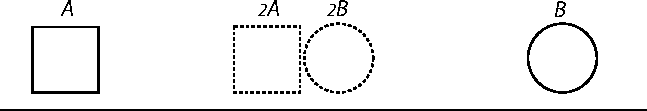
\includegraphics[width=0.75\textwidth]{gesamttex/edit_VIII,3/images/LH_37_05_150-151_d1_150v.pdf}} 
\vspace{0.5em}
\centerline{\lbrack\textit{Fig.~1}\rbrack}
% \newpage%
\vspace{1.2em}
\pstart
Si duo corpora sibi occurant, in momento concursus\protect\index{Sachverzeichnis}{momentum concursus} unumquodque duos
% =
habet conatus, unum proprium\protect\index{Sachverzeichnis}{conatus proprius} alterum acceptum\protect\index{Sachverzeichnis}{conatus acceptus}. Conatus autem proprii sunt impossibiles,
% =
quia tendunt ad penetrationem, restant ergo tantum
%
\edtext{accepti, ac proinde}{\lemma{accepti,}\Bfootnote{\textit{(1)}~id est unum corpus alterius conatum \textit{(2)}~ac proinde~\textit{L}}}
%
permutantur conatus, id est corpus unum alterius potentiam\protect\index{Sachverzeichnis}{potentia} 
% =
et directionem recipit. Nec dici potest conatus proprios\protect\index{Sachverzeichnis}{conatus proprius} jam esse
% =
destructos per aequales contrarios acceptos\protect\index{Sachverzeichnis}{conatus acceptus} (\phantom)\hspace*{-1.2mm}posito corpora esse aequivelocia 
% =
et aequalia\phantom(\hspace*{-1.2mm}) quia duo conatus contrarii aequales\protect\index{Sachverzeichnis}{conatus contrarius aequalis} consistere possunt, faciunt enim 
% =
quietem, at vero non possunt consistere conatus, qui simul positi inducerent 
% =
penetrationem. Duae tamen supersunt difficultates quae impediunt 
% =
quominus hanc ratiocinationem pro demonstratione habeam, una quod duo 
% =
\edtext{conatus contrarii proprius et acceptus aequales simul stantes,}{\lemma{conatus}\Bfootnote{\textit{(1)}~proprii et accepti \textit{(2)}~contrarii proprius et acceptus \textbar\ aequales \textit{erg.}\ \textbar\ simul stantes,~\textit{L}}}
%
faciunt ut corpus
%
non exeat loco,
% =
altera quod non video quomodo corpus in aliud agat momento concursus\protect\index{Sachverzeichnis}{momentum concursus}, nisi in eo proprium
% =
suum conatum habeat. Dicendumne eo momento quo in aliud agit nondum alterius conatum
% =
accepisse, sed accipere nunc primum, eo tempore quo dat suum. Ita est. Sed ubi dedit suum,
% =
videtur non amplius habere, quia vires\protect\index{Sachverzeichnis}{vis} augeri non possunt. Quod principium aliunde assumendum
% =
est, alioqui corpus majus quiescens totam celeritatem minoris reciperet.
\pend\pstart
Phaenomena\protect\index{Sachverzeichnis}{phaenomenon} quae fiunt in corporibus sensibilibus\protect\index{Sachverzeichnis}{corpus sensibile}, ideo longe alia sunt, quia corpora 
% =
sensibilia\protect\index{Sachverzeichnis}{corpus sensibile} 
%
\edtext{omnia}{\lemma{}\Bfootnote{omnia \textit{erg.}\ ~\textit{L}}}
%
flexibilia sunt.  
\pend\pstart
Necessarium est, ut partes solae cedant non tota, quando vis unionis\protect\index{Sachverzeichnis}{vis unionis} superatur 
% =
alioqui licet partiri vellemus actionem, nihilominus maxima corpora sensibilia\protect\index{Sachverzeichnis}{corpus sensibile} a minimis moverentur 
% =
aut sisterentur.
\pend
\newpage
\pstart
%
%\hspace{1mm}\hspace{-1mm}% Trick, weil \edlabel nicht zu \par-Beginn sein darf
%
Ponamus \edlabel{37_05_150-151_4a}corpora concurrentia esse perfecte Elastica\protect\index{Sachverzeichnis}{corpus perfecte elasticum}, seu ita flexibilia\protect\index{Sachverzeichnis}{corpus flexibile}, ut totam vim 
% =
acceptam\protect\index{Sachverzeichnis}{vis accepta} restituendo reddant, nihilque ejus in minutis suis partibus 
%
\edtext{}{% NEUER ABSATZ UND VARIANTEN – "perdant."
{\xxref{37_05_150-151_2a}{37_05_150-151_2b}}%
\lemma{perdant.}%
\Bfootnote{\textit{(1)}~Concursu duplex exercetur vis, una in corpora, tendens ad eorum propulsionem \textit{(2)}~Ictus totus \textit{(3)}~Tota potentia \textit{(a)}~corporibus \textit{(b)}~corporis~\textit{L}}}% 
\edlabel{37_05_150-151_2a}perdant.
\pend \pstart
Tota potentia\protect\index{Sachverzeichnis}{potentia} corporis \edlabel{37_05_150-151_2b}
%
incurrentis transfertur in corpus accipiens, sed 
%
quia %			
% =
corpus accipiens est flexile,
%
\edtext{hinc non totum}{\lemma{hinc}\Bfootnote{\textit{(1)}~eo usque \textit{(2)}~non totum~\textit{L}}} 
%
propellitur, sed ictu accepto\protect\index{Sachverzeichnis}{ictus acceptus} eousque
% =
flectitur, donec debilior fiat ictus acceptus\protect\index{Sachverzeichnis}{ictus acceptus}, quam ut porro amplius flectere possit, residuum % =
ergo impetus accepti\protect\index{Sachverzeichnis}{impetus acceptus} impenditur in totius corporis propulsionem.
%
Nimirum corporis 
% =
portio prior quae ictum recepit, ruit in sequentem, et sese continuo premunt, donec 
% =
non amplius possint, resistente fortius corporis compage, et tunc resistenti, id est reliquo,
% =
id est nunc ob connexionem redditam, toti, ictum tunc imprimunt. Eo porro momento
% =
tota corpora quiescunt, quo durante fit flexio\protect\index{Sachverzeichnis}{flexio}, cessante flexione\protect\index{Sachverzeichnis}{flexio} incipiunt motum, seu ictu
% =
residuo aguntur. Ponamus 
%
\edtext{jam corporis \textit{A}}{\lemma{jam corporis}\Bfootnote{\textit{(1)}~\textit{a}, vim esse \textit{ae}, quam dedit \textit{(2)}~\textit{A}~\textit{L}}}
%
vim primam fuisse
% =
\textit{ae}, corporis \textit{B}, vim \textit{bf}. 
%
\edtext{Erit vis in corpore}{\lemma{Erit vis}\Bfootnote{\textit{(1)}~corporis \textit{(2)}~in corpore~\textit{L}}}
%
\textit{A} recepta\protect\index{Sachverzeichnis}{vis in corpore recepta} \textit{bf}, et vis in corpore \textit{B} recepta\protect\index{Sachverzeichnis}{vis in corpore recepta} \textit{ae}. 
% =
Sit %	
%
vis quae flexioni\protect\index{Sachverzeichnis}{flexio} impenditur 
%
\edtext{$d^2$, tam}{\lemma{$d^2$,}\Bfootnote{\textit{(1)}~reliqua ergo vi \textit{(2)}~tam~\textit{L}}}
%
in \textit{A}, quam in \textit{B}, quia ponuntur ejusdem
%
\edtext{materi\lbrack ae\rbrack,}{\lemma{}\Bfootnote{materia \textit{L}\ \textit{ändert Hrsg.}}} quia ergo reliqua est vis
%
\edtext{propellens\protect\index{Sachverzeichnis}{vis propellens}, ideo}{\lemma{propellens,}\Bfootnote{\textit{(1)}~erit \textit{(2)}~ideo~\textit{L}}}
%
\textit{A} propelletur vi 
%
$bf-d^2$ et \textit{B} vi $ae - d^2$.
%
Vis autem flexionis\protect\index{Sachverzeichnis}{vis flexionis} in utroque est $2d^2$.
%
Restitutione flexorum ad corpora porro propellenda nihil 
%%%%%%%%%%%%%%%%%%%%%%%%%%%%%%%%%%%%%%%%%%%%%%%%%%%%%%%%%%%%%%%%%%%%
%%%%%%%%%%%%%%%%%   F. 150 V.         %%%%%%%%%%%%%%%%%%%%%%%%%%%%%%
%%%%%%%%%%%%%%%%%%%%%%%%%%%%%%%%%%%%%%%%%%%%%%%%%%%%%%%%%%%%%%%%%%%%
\lbrack151~r\textsuperscript{o}\rbrack\
plane contribuetur, quia vis $2d^2$ in corpora distributa aequaliter, quia aequalia sunt,
% =
ea tantum denuo flectet, nempe reddetur unicuique flexio\protect\index{Sachverzeichnis}{flexio} $d^2$, quae non propellet,
% =
\edtext{quia jam,}{\lemma{quia}\Bfootnote{\textit{(1)}~subj \textit{(2)}~non \textit{(3)}~ut \textit{(4)}~jam,~\textit{L}}}
%
ex hypothesi semel sine impulsu recepta est. His
% =
ita positis dicendum esset, ideo visum fuisse in duris
%
\edtext{vim permutari}{\lemma{vim}\Bfootnote{\textit{(1)}~remanere \textit{(2)}~permutari~\textit{L}}}
%
exacte
% =
quia $d^2$ est valde parva. Patet etiam quod $d^2$ sit eadem quantuscunque sit ictus
%
\edtext{incussus. Imo}{\lemma{incussus}\Bfootnote{\textit{(1)}~, ideoque \textit{(2)}~. Imo~\textit{L}}}
%
non ita. Sed tanta foret semper vis propellens\protect\index{Sachverzeichnis}{vis propellens}, quanta est corporis
% =
ad fractionem\protect\index{Sachverzeichnis}{resistentia ad fractionem} seu flexum majorum resistentia\protect\index{Sachverzeichnis}{resistentia ad flexum}.\edlabel{37_05_150-151_4b}
\pend\pstart
Superest \edtext{difficultas. Talia}{\lemma{}\Bfootnote{difficultas. \textit{(1)}~Non \textit{(2)}~Talia~\textit{L}}} quidem procederent, si corpus inflexile\protect\index{Sachverzeichnis}{corpus inflexile} in Elasticum\protect\index{Sachverzeichnis}{corpus elasticum} 
% =
impingeret, id enim totam statim daret ei vim suam. Sed cum corpora sunt
% =
Elastica, videntur prima occurrentia sibi tantum vim quam habent mutuo communicare, et
% =
in sequentes 
%
suas compartes ruere quae etiam vim communicant cum ipsa adveniunt et
% =
si medio tempore resilirent, tamen rursus in se ipsa mutuo impingerentur atque iterum
% =
eodem modo reflecterentur, interea reliquum sequitur, etiamque ad ictum venit, idemque iterum
% =
contingit, atque ita porro sibi ita appropinquant, atque in se mutuo invadunt atque ingrediuntur,
% =
donec major sit vis unionis\protect\index{Sachverzeichnis}{vis unionis} in corpore, quam ut  
%
\edtext{cedat residuae vi,\protect\index{Sachverzeichnis}{vis residua}}{\lemma{cedat}\Bfootnote{\textit{(1)}~residuis corporis \textit{(2)}~residuae vi,~\textit{L}}}
%
id est flectetur donec flecti amplius non possit ab hac quidem vi, sed potius tota utrobique
% =
sentiunt ictum. Hoc intelligendum hoc modo\lbrack:\rbrack\ partes a potentiis\protect\index{Sachverzeichnis}{potentia} partium flectuntur, 
% =
partes autem simul sumendae semper fiunt  
%
\edtext{majores, donec}{\lemma{majores,}\Bfootnote{\textit{(1)}~quia \textit{(2)}~donec~\textit{L}}}
%
tandem totum simul
% =
sit sumendum, partibus amplius flecti nolentibus, quo facto 
%
\edtext{resilientibus}{\lemma{resilientibus}\Bfootnote{\textit{(1)}~corporibus \textit{(2)}~partibus~\textit{L}}}
%
partibus rursus eadem vis accepta\protect\index{Sachverzeichnis}{vis accepta} mutuo redditur, itaque ea vis tantum permuta\textlangle tur.\textrangle\ 
% =
Sed quoniam omnis illa vis flexionum\protect\index{Sachverzeichnis}{vis flexionis}, causat tantum flexiones\protect\index{Sachverzeichnis}{flexio}, quoniam sine totius
% =
impulsu causare potest, ideo perditur, et corpora tantum a se invicem ea vi, quae 
% =
flexionibus\protect\index{Sachverzeichnis}{flexio} superfuit separantur. Sonus\protect\index{Sachverzeichnis}{sonus} nihil aliud est, quam illae vibrationes atque saepe
% =
repetitae percussiones, cumque vis soni non sit exigua, et satis late propagetur, mirum
% =
non est tantum perdi. Quo duriora sunt corpora hoc minus videtur perdi, magis enim
% =
resistunt flexioni\protect\index{Sachverzeichnis}{flexio}. 
\pend
%%%%%%%%%%%%%%%%%%%%%%%%%%%%%%%%%%%%%%%%%%%%%%%%%%%%%%%%%%%%%%%%%%%%% 
%%%%%%%%%%%%%%%%%%%%         FIG 2.     %%%%%%%%%%%%%%%%%%%%%%%%%%%%%    
%%%%%%%%%%%%%%%%%%%%%%%%%%%%%%%%%%%%%%%%%%%%%%%%%%%%%%%%%%%%%%%%%%%%% 
% \newpage%
\vspace{2.0em}
\centerline{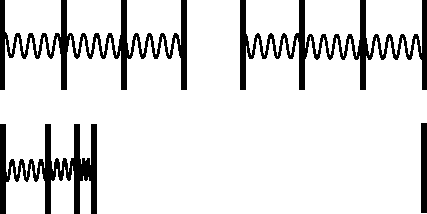
\includegraphics[width=0.33\textwidth]{gesamttex/edit_VIII,3/images/LH_37_05_150-151_d2_151r.pdf}} 
\vspace{0.5em}
\centerline{\lbrack\textit{Fig.~2}\rbrack}
% \newpage%
\vspace{2.0em}
\centerline{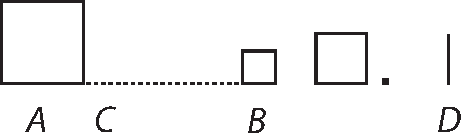
\includegraphics[width=0.33\textwidth]{gesamttex/edit_VIII,3/images/LH_37_05_150-151_d3_151r.pdf}} 
\vspace{0.5em}
\centerline{\lbrack\textit{Fig.~3}\rbrack}
% \newpage%
\vspace{1.5em}
%  
%
\pstart
Considerandum et 
%
\edtext{dum anterior}{\lemma{dum}\Bfootnote{\textit{(1)}~unum \textit{(2)}~anterior~\textit{L}}}
%
corporis pars rejicitur, posteriorem
% =
nihilominus progredi, quod tensionem auget.
\\\indent Utile erit instructos vesicis\protect\index{Sachverzeichnis}{vesica} praefixis inflatisque
% =
currus\protect\index{Sachverzeichnis}{currus} duos concurrere, ut appareat ad oculum progressus actionis\protect\index{Sachverzeichnis}{progressus actionis}. 
% =
Certum est duo corpora elastica\protect\index{Sachverzeichnis}{corpus elasticum} ita concurrentia, ut \lbrack\textit{Text bricht ab.}\rbrack 
\pend \pstart
Positis duobus principiis uno de centro gravitatis\protect\index{Sachverzeichnis}{centrum gravitatis} recta procedente, altero de eadem potentia\protect\index{Sachverzeichnis}{potentia} servata, 
% = 
difficile videtur omnia cum phaenomenis\protect\index{Sachverzeichnis}{phaenomenon} conciliare, quia enim necesse est corpora omnia utcunque mota semper eundem 
% =
servare centri motum, hinc suppositis licet corporibus concurrentibus elasticis; poterimus elasticam vim\protect\index{Sachverzeichnis}{vis elastica} repraesentare
% =
ponderibus (non in ipso corpore, sed alio) suspensis per subtilissima fila, quae pondera postea rursus decidunt, cum fit restitutio\protect\index{Sachverzeichnis}{restitutio}, quo 
% =
facto patet pondera quippe rursus decidentia nihil circa centri totalis situm variare, non magis quam si 
% =
immobilia mansissent, adeoque in aggregato duorum corporum et partium ex quibus componentur, non obstantibus omnibus hoc 
% =
observari, ut semper eodem modo procedat centrum gravitatis\protect\index{Sachverzeichnis}{centrum gravitatis}. 
%
Et quamvis vis nonnihil diminuatur, id tamen
% =
%%%%%%%%%%%%%%%%%%%%%%%%%%%%%%%%%%%%%%%%%%%%%%%%%%%%%%%%%%%%%%%%%%%%% 
%%%%%%%%%%%%%%%%%%%%         FIG 3.     %%%%%%%%%%%%%%%%%%%%%%%%%%%%%    
%%%%%%%%%%%%%%%%%%%%%%%%%%%%%%%%%%%%%%%%%%%%%%%%%%%%%%%%%%%%%%%%%%%%% 
nihil impedit, quominus corpus magnum semper quiescat, et parvum totam ejus vim accipiat. 
% =
Quod ab experientia est alienum; nec video quod possit responderi. Videndum an non 
% =
necesse sit potius, non centrum gravitatis\protect\index{Sachverzeichnis}{centrum gravitatis}, sed centrum potentiae\protect\index{Sachverzeichnis}{centrum potentiae} semper in eadem  
% =
\edtext{recta procedere}{\lemma{recta}\Bfootnote{\textit{(1)}~descendere \textit{(2)}~pr \textit{(3)}~procedere~\textit{L}}}: 
%
Tunc corpus magnum impingens in parvum minime quiescet\lbrack,\rbrack\
% =
nam quia uno posito corpore quiescente, altero moto, centrum poten\lbrack151~v\textsuperscript{o}\rbrack tiae semper incidit in ipsum centrum gravitatis\protect\index{Sachverzeichnis}{centrum gravitatis} corporis moti, (\phantom)\hspace*{-1.2mm}ob infinitam potentiae\protect\index{Sachverzeichnis}{potentia} ejus ad quiescentis 
% =
potentiam\protect\index{Sachverzeichnis}{potentia} rationem\phantom(\hspace*{-1.2mm}) ideo cum manifestum sit corpus parvum impulsum 
% 
\edtext{debere celerius}{\lemma{debere}\Bfootnote{\textit{(1)}~celeriter \textit{(2)}~celerius~\textit{L}}}
%
moveri
% =
quam ante magnum (in reciproca corporum ratione), si eadem vis manere et magnum post 
% =
impulsum quiescere debet, hinc sequeretur centrum illud potentiae\protect\index{Sachverzeichnis}{centrum potentiae}
%
\edtext{quod cum magno}{\lemma{quod cum}\Bfootnote{\textit{(1)}~parvo venit \textit{(2)}~magno~\textit{L}}}
% =
tarde venit, cum parvo in eadem recta celerius progredi, contra hypothesin. Si duo corpora
% =
concurrant reciproca celeritate, centrum potentiae\protect\index{Sachverzeichnis}{centrum potentiae} erit manebitque in medio, et redibunt ea celeritate
% =
qua venere. Si corpus incurrat in aequale  
%
\edtext{quiescens; tunc}{\lemma{quiescens;}\Bfootnote{\textit{(1)}~centrum \textit{(2)}~tunc~\textit{L}}}
%
quiescet in ejus loco, et ipsum 
% =
motum eadem celeritate progredietur; ita enim etiam centrum potentiae\protect\index{Sachverzeichnis}{centrum potentiae} in eadem recta progredietur.
% =
Si duo corpora aequalia concurrant in eadem 
%
\edtext{recta, diversis}{\lemma{recta}\Bfootnote{\textit{(1)}~unum \textit{(2)}~, tunc \textit{(3)}~, diversis~\textit{L}}} 
%
celeritatibus, tunc 
% =
si unum alteri suam det vim, patet illas celeritates sumi posse pro
%
\edtext{corporibus, diversis eodem modo, sed aequaliter}{\lemma{corporibus,}\Bfootnote{\textit{(1)}~at ideo ea \textit{(2)}~diversis eodem modo, \textbar\ sed \textit{erg.}\ \textbar\ aequaliter~\textit{L}}} 
%
motis.
\pend
%
%%%%%%%%%%%%%%%%%%%%%%%%%%%%%%%%%%%%%%%%%%%%%%%%%%%%%%%%%%%%%%%%%%%%% 
%%%%%%%%%%%%%%%%%%%%         FIG 4.     %%%%%%%%%%%%%%%%%%%%%%%%%%%%%    
%%%%%%%%%%%%%%%%%%%%%%%%%%%%%%%%%%%%%%%%%%%%%%%%%%%%%%%%%%%%%%%%%%%%% 
% \newpage%
\vspace{2.0em}
\centerline{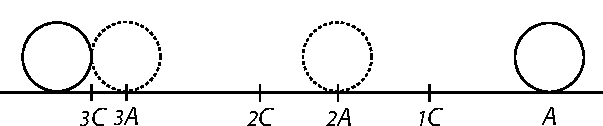
\includegraphics[width=0.5\textwidth]{gesamttex/edit_VIII,3/images/LH_37_05_150-151_d4_151v.pdf}} 
\vspace{0.5em}
\centerline{\lbrack\textit{Fig.~4, gestr.}\rbrack}
 \newpage%
%\vspace{1.5em}
% 
\centerline{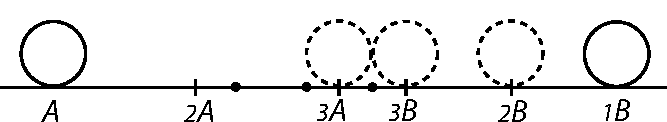
\includegraphics[width=0.55\textwidth]{gesamttex/edit_VIII,3/images/LH_37_05_150-151_d5_151v.pdf}}
\vspace{0.5em}
\centerline{\lbrack\textit{Fig.~5}\rbrack}
% \newpage%
\vspace{2.5em}
%
\centerline{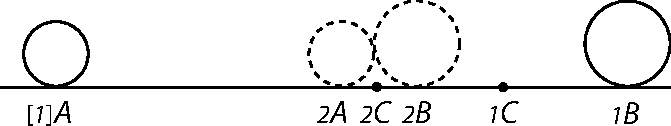
\includegraphics[width=0.55\textwidth]{gesamttex/edit_VIII,3/images/LH_37_05_150-151_d6_151v.pdf}}
\vspace{0.5em}
\centerline{\lbrack\textit{Fig.~6}\rbrack}
% \newpage%
\vspace{1.5em}
%
\pstart
\edtext{}{\lemma{\hspace*{1,6mm}\lbrack\textit{Fig.~5}\rbrack}\killnumber\Cfootnote{Ein gestrichener Entwurf zum Diagramm wird nicht wiedergegeben.}}
$ae+bf \sqcap ai+bm$. Seu $ae-ai \sqcap bm-bf$. Seu $\displaystyle\frac{a}{b} \sqcap \displaystyle\frac{m-f}{e-i}$.
\pend\pstart
% =
\rule[0cm]{0mm}{16pt}$\displaystyle\frac{{\scriptstyle \textit{1}}B{\scriptstyle \textit{1}}C}{{\scriptstyle \textit{1}}A{\scriptstyle \textit{1}}C} \sqcap \displaystyle\frac{ae}{bf} \sqcap \displaystyle\frac{{\scriptstyle \textit{2}}B{\scriptstyle \textit{2}}C}{{\scriptstyle \textit{2}}A{\scriptstyle \textit{2}}C}.$
%
\pend\pstart
\rule[0cm]{0mm}{18pt}$\displaystyle\frac{{\scriptstyle \textit{2}}B{\scriptstyle \textit{2}}C \sqcap d^2}{{\scriptstyle \textit{2}}A{\scriptstyle \textit{2}}C \sqcap d^2\; \displaystyle\frac{bf}{ae}}$. ${\scriptstyle \textit{1}}A{\scriptstyle \textit{2}}A \sqcap el$. ${\scriptstyle \textit{1}}B{\scriptstyle \textit{2}}B \sqcap fl$. \edtext{${\scriptstyle \textit{1}}C{\scriptstyle \textit{2}}C \sqcap c^2$.}{\lemma{}\Bfootnote{{${\scriptstyle \textit{1}}C{\scriptstyle \textit{2}}C \sqcap c^2$.\ \textit{erg.}~\textit{L}}}}
\pend\pstart
\rule[0cm]{0mm}{20pt}%
${\scriptstyle \textit{1}}B{\scriptstyle \textit{2}}C \sqcap \begin{array}{c} 
ae\\ {\scriptstyle \textit{1}}B{\scriptstyle \textit{1}}C\end{array} \pleibdashv\ 
\begin{array}{c} 
c^2\\ {\scriptstyle \textit{1}}C{\scriptstyle \textit{2}}C \end{array} \sqcap
\begin{array}{c} 
fl\\ {\scriptstyle \textit{1}}B{\scriptstyle \textit{2}}B \end{array} + 
\begin{array}{c} 
d^2\\ {\scriptstyle \textit{2}}B{\scriptstyle \textit{2}}C \end{array}.$
Ergo
$\begin{array}{r}
d^2\\
{\scriptstyle \textit{2}}B{\scriptstyle \textit{2}}C
\end{array} \sqcap ae\ \pleibdashv\ c^2 - fl$
et
${\begin{array}{r} %Hier habe ich die Gleichung eingeklammert, damit sie nicht über zwei Zeilen gespalten wird
{\scriptstyle \textit{2}}A{\scriptstyle \textit{2}}C\\
d^2\displaystyle\frac{bf}{ae}
\end{array}
\sqcap bf\, \leibdashv\ \displaystyle\frac{c^2bf}{ae}-\displaystyle\frac{bf^2l}{ae}}.$
%Zeichen in der Mitte - Gleichung in A
\pend\pstart
${\scriptstyle \textit{1}}A{\scriptstyle \textit{2}}C \sqcap \begin{array}{c} 
bf\\ {\scriptstyle \textit{1}}A{\scriptstyle \textit{1}}C\end{array} \pleibdashv\ 
\begin{array}{c} 
c^2\\ {\scriptstyle \textit{1}}C{\scriptstyle \textit{2}}C \end{array} \sqcap
\begin{array}{c} 
el\\ {\scriptstyle \textit{1}}A{\scriptstyle \textit{2}}A \end{array} + 
\begin{array}{c} 
\displaystyle\frac{d^2bf}{ae}\\ {\scriptstyle \textit{2}}A{\scriptstyle \textit{2}}C \end{array}.$
Ergo
$\displaystyle\frac{d^2bf}{ae} \sqcap bf\, \pleibvdash\ c^2 - el$
\pend\pstart 
%%%
idem super 
$\sqcap\, bf\, \pleibdashv\ \displaystyle\frac{c^2bf}{ae}-\displaystyle\frac{bffl}{ae}$ erit 
$\pleibdashv\ c^2\; \overline{bf+ae} \sqcap \displaystyle\frac{-ae^2l+bf^2l}{bf+ae}.$
\pend
\newpage
\pstart
\rule[0cm]{0mm}{10pt}Ubi notandum elegans theorema\protect\index{Sachverzeichnis}{theorema elegans} 
%
obiter, si sit $a\sqcap b$ fore viam centri potentiae\protect\index{Sachverzeichnis}{via centri potentiae} $\overline{-e+f}\;l$ 
seu differentiam 
%
\edtext{%
\edtext{celeritatum.}{%
\lemma{}%
\Afootnote{%
\textit{Zwischen den Zeilen, über} celeritatum:\enspace %
viarum corporum\protect\index{Sachverzeichnis}{via corporis}}}
%
Idque}{\lemma{celeritatum.}\Bfootnote{\textit{(1)}~Hinc necesse est, ut \textit{(2)}~Idque~\textit{L}}}   
%
fit, cum reciprocantur celeritates, manet 
% =
enim eadem \edtext{differenti\lbrack a\rbrack}{\lemma{}\Bfootnote{differentiam \textit{L}\ \textit{ändert Hrsg.}}} 
%
viarum corporum\protect\index{Sachverzeichnis}{via corporis} seu 
% 
celeritatum. Idem est quando
%
$bf \sqcap ae$.
% =
Ergo his duobus casibus, id est quando corpora duo sunt aequalia, et quando sunt celeritates 
% =
reciproce proportionales corporibus, tunc mea Hypothesis\protect\index{Sachverzeichnis}{hypothesis mea} 
%
\edtext{Hugenianae\protect\index{Namensregister}{\textso{Huygens} (Hugenius, Ugenius, Hugens, Huguens), Christiaan 1629\textendash1695}\protect\index{Sachverzeichnis}{hypothesis Hugeniana}}{%
\lemma{Hugenianae}%
\Cfootnote{%
\protect\index{Namensregister}{\textso{Huygens} (Hugenius, Ugenius, Hugens, Huguens), Christiaan 1629\textendash1695}\textsc{C.~Huygens}, \cite{00529}\glqq Regles du mouvement dans la rencontre des corps\grqq, \cite{00157}\textit{JS} (Pariser Ausgabe), 18.~März 1669, S.~22\textendash24 (\cite{00113}\textit{HO} XVI, S.~179\textendash181).
}} 
%
consentit. Nunc 
% =
ut generaliter eadem semper sit celeritas centri potentiae, debet esse
%
\rule[0cm]{0mm}{18pt}$\displaystyle\frac{-ae^2+bf^2}{bf+ae} \sqcap \displaystyle\frac{(\leibdashv)\, ai^2\, \leibvdash\, bm^2}{bm+ai}$. 
%
Ponendo scil. \textit{i} pro celeritate posteriore ipsius \textit{a}, et \textit{m}
% =
\rule[0cm]{0mm}{10pt}pro celeritate posteriore ipsius \textit{b}. Et quia super diximus esse $bf+ae \sqcap bm + ai$, ideo
% =
ob aequalem fractionem et aequales nominatores erunt et numeratores aequales, sive erit:
% =
$-ae^2 + bf^2 \sqcap (\pleibdashv)\,ai^2\, (\pleibvdash)\, bm^2$. Et transponendo 
%
$+ae^2\, \edtext{(\lbrack\pleibdashv\rbrack)\,ai^2}{\lemma{\pleibvdash}\Bfootnote{\textit{L}\ \textit{ändert Hrsg.}}} \sqcap +bf^2\, (\pleibdashv)\,bm^2$ 
%
seu erit
%
$\displaystyle\frac{a}{b} \sqcap \displaystyle\frac{f^2\,(\leibdashv)\,m^2}{e^2-i^2}$
%
at idem
%
$\sqcap\, \displaystyle\frac{m-f}{e-i}$.
%
Ergo
%
$\displaystyle\frac{a}{b} \sqcap \displaystyle\frac{m+f}{e+i}$.
%
Ergo quando eadem
% =
est via centri gravitatis\protect\index{Sachverzeichnis}{via centri gravitatis}, 
%
\rule[0cm]{0mm}{12pt}eadem est quoque via centri potentiae\protect\index{Sachverzeichnis}{via centri potentiae}, tametsi hae duae viae non sint 
% =
eadem inter se. Imo aliquando maximum est discrimen, scilicet tunc cum fit \textit{el} quantitas
% =
\rule[0cm]{0mm}{18pt}negativa, posito enim $E \sqcap -e$, fiet: 
%
$c^2 \sqcap \displaystyle\frac{+aE^2l+bf^2l}{bf+ae}$.%
%
\edlabel{37_05_150-151_3a}\edtext{}{% C-Footnote (Huygens-Stelle) um eine B-Footnote herum (Stufen)
{\xxref{37_05_150-151_3a}{37_05_150-151_3b}}%
\lemma{Et \lbrack...\rbrack\ quadrata}\Cfootnote{\cite{00529}a.a.O., §6, S.~23.}} 
%
Et tunc verum erit quod dixit 
%
\rule[0cm]{0mm}{9pt}Hugenius\protect\index{Namensregister}{\textso{Huygens} (Hugenius, Ugenius, Hugens, Huguens), Christiaan 1629\textendash1695} universaliter esse verum, quod aequale semper factum \edtext{ex corporibus}{\lemma{ex}\Bfootnote{\textit{(1)}~partem \textit{(2)}~corporibus~\textit{L}}} in celeritatum quadrata.%
\edlabel{37_05_150-151_3b}
% =
Ergo modo summa horum modo differentia eadem.
%
Mirum Hugenium\protect\index{Namensregister}{\textso{Huygens} (Hugenius, Ugenius, Hugens, Huguens), Christiaan 1629\textendash1695} dixisse
tam uno quam altero casu vera, neutra suis principiis consona, fuit propinquus veritati, sed nescio quomodo seductus.
%
\edtext{Non debebat autem %	C-Fn Huygens um B-Fn herum
\edtext{negare summas}{\lemma{negare}%
\Bfootnote{\textit{(1)}~factu \textit{(2)}~ex corpori \textit{(3)}~summas~\textit{L}}} %
ex factis corporum in suas celeritates esse semper aequales.}{%
\lemma{Non \lbrack...\rbrack\ aequales}%
\Cfootnote{%
\cite{00529}a.a.O., §5, S.~23.}} %
Poterant enim 
% =
simul stare.\pend
\count\Bfootins=1200%
\count\Afootins=1200%
\count\Cfootins=1200
